	

\begin{table}[h!]
\section{Integralrechnung}

\begin{center}


% % % % % % % % % % % % % % % % % %
%Ableitungstabelle
% % % % % % % % % % % % % % % % % %	
\begin{tabularx}{540pt}{|X|X||X|X|}	
	\hline
	\rowcolor{Gray}
	\multicolumn{4}{|c|}{\textbf{Darstellungsformen}}\\
	\hline
	
	Funktion & Ableitung & Funktion & Ableitung \\
	\hline
	$(uv)'$ & $u'v+ uv'$ & 
    $\bigg(\dfrac{u}{t} \bigg)'$& $\bigg(\dfrac{u't-ut'}{t^2}\bigg) $ \\
	\hline
	$(u^v)'$ & $u^v\bigg(v' \ln(u) + \dfrac{vu'}{u} \bigg)$  & 
	$a^x$ & $a^x \cdot \ln(a)$\\
	\hline
	$arcsin(x)$& $\dfrac{1}{\sqrt{1-x^2}}$&
	$arcos(x)$& $-\dfrac{1}{\sqrt{1-x^2}}$\\
	\hline
	$arctan(x)$& $\dfrac{1}{1+x^2}$&
	$arccot(x)$& $-\dfrac{1}{1+x^2}$\\
	\hline	
	$arsinh(x)$& $\dfrac{1}{\sqrt{x^2+1}}$&
	$arcosh(x)$& $\dfrac{1}{\sqrt{x^2-1}}$\\
	\hline	
	$artanh(x)$& $\dfrac{1}{1-x^2}$&
	$arcoth(x)$&$\dfrac{1}{1-x^2}$\\
	\hline
	$tanh(x)$  &$\dfrac{1}{cosh^2(x)}=1-tanh(x)^2$&
	& \\
\end{tabularx}


% % % % % % % % % % % % % % % % % %
%Arten der Integration
% % % % % % % % % % % % % % % % % %	
\begin{tabularx}{540pt}{|p{150pt}|X|}
		\hline
		\rowcolor{Gray} 
		\multicolumn{2}{|c|}{\textbf{Integrationsmethoden}}	\\
		\hline
		
		Linearität & $\int{f(\alpha x+\beta )dx=\dfrac{F(\alpha x+
						\beta)}{\alpha} +C}$  \\
		\hline
		
		Partielle Integration&  $\int\limits_a^b{u'(x)\cdot v(x)dx}=\biggl[ u(x)\cdot v(x) \biggr]_a^b
	 	   -\int\limits_a^b{u(x)\cdot v'(x)dx}$  \\
		\hline
		Rationalisierung& $ t=\tan\frac{x}{2}, \qquad dx=\frac{2dt}{1+t^2} \qquad 
		 	   \sin  x=\frac{2t}{1+t^2} \qquad  \cos x=\frac{1-t^2}{1+t^2}
		 	   \newline  \quad\int{R(\sin(x)\cos(x))dx}$ \\
		\hline
		Substitution& $\int\limits_{a}^{b}{f(x)dx}=\int\limits_{g^{-1}(a)}^{g^{-1}(b)}{f(g(t))\cdot
			g'(t)dt}\qquad t=g^{-1}(x)\qquad 
			\newline \fbox{x=g(t)}\qquad dx=g'(t)\cdot dt$ \\
		\hline
		Logarithmische& $ \int{\frac{f'(x)}{f(x)}dx}=\ln|f(x)|+C	\qquad{(f(x)\neq 1)}$ \\
		\hline
		Potenzregel& $\int{f'(x)\cdot (f(x))^{\alpha} dx}= \dfrac{f(x)^{\alpha +1}}{\alpha+1}+C \qquad{(\alpha \neq -1)}$ \\
		\hline
		Differentiation&$\int \limits ^{b} _{a} {f'(t)dt}=f(b)-f(a)
					\newline   \frac{d}{dx} \int \limits ^{x} _{1} {f(t)dt}=f(x)$\\
		\hline
\end{tabularx}
\end{center}
\end{table}

%neue Seite

\begin{table}[h!]
\begin{center}

% % % % % % % % % % % % % % % % % %
%Uneigentliche Integrale
% % % % % % % % % % % % % % % % % %	
\begin{tabularx}{540pt}{|p{270pt}|X|}
	\hline
	\rowcolor{Gray}
	\multicolumn{2}{|c|}{\textbf{Uneigentliche Integrale}}\\
	\hline

	Für unbeschränkte Funktionen & Für unbeschränkte Grenzen\\
	
	\hline
		\raisebox{-.8\totalheight}{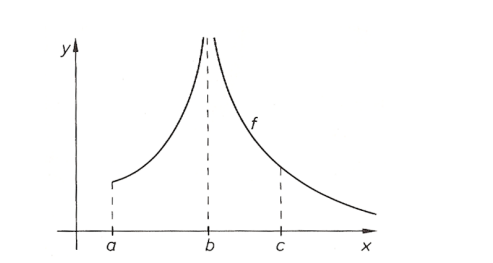
\includegraphics[width = 4cm]{bilder/1_unbeschrfkt.png}} & \raisebox{-.8\totalheight}{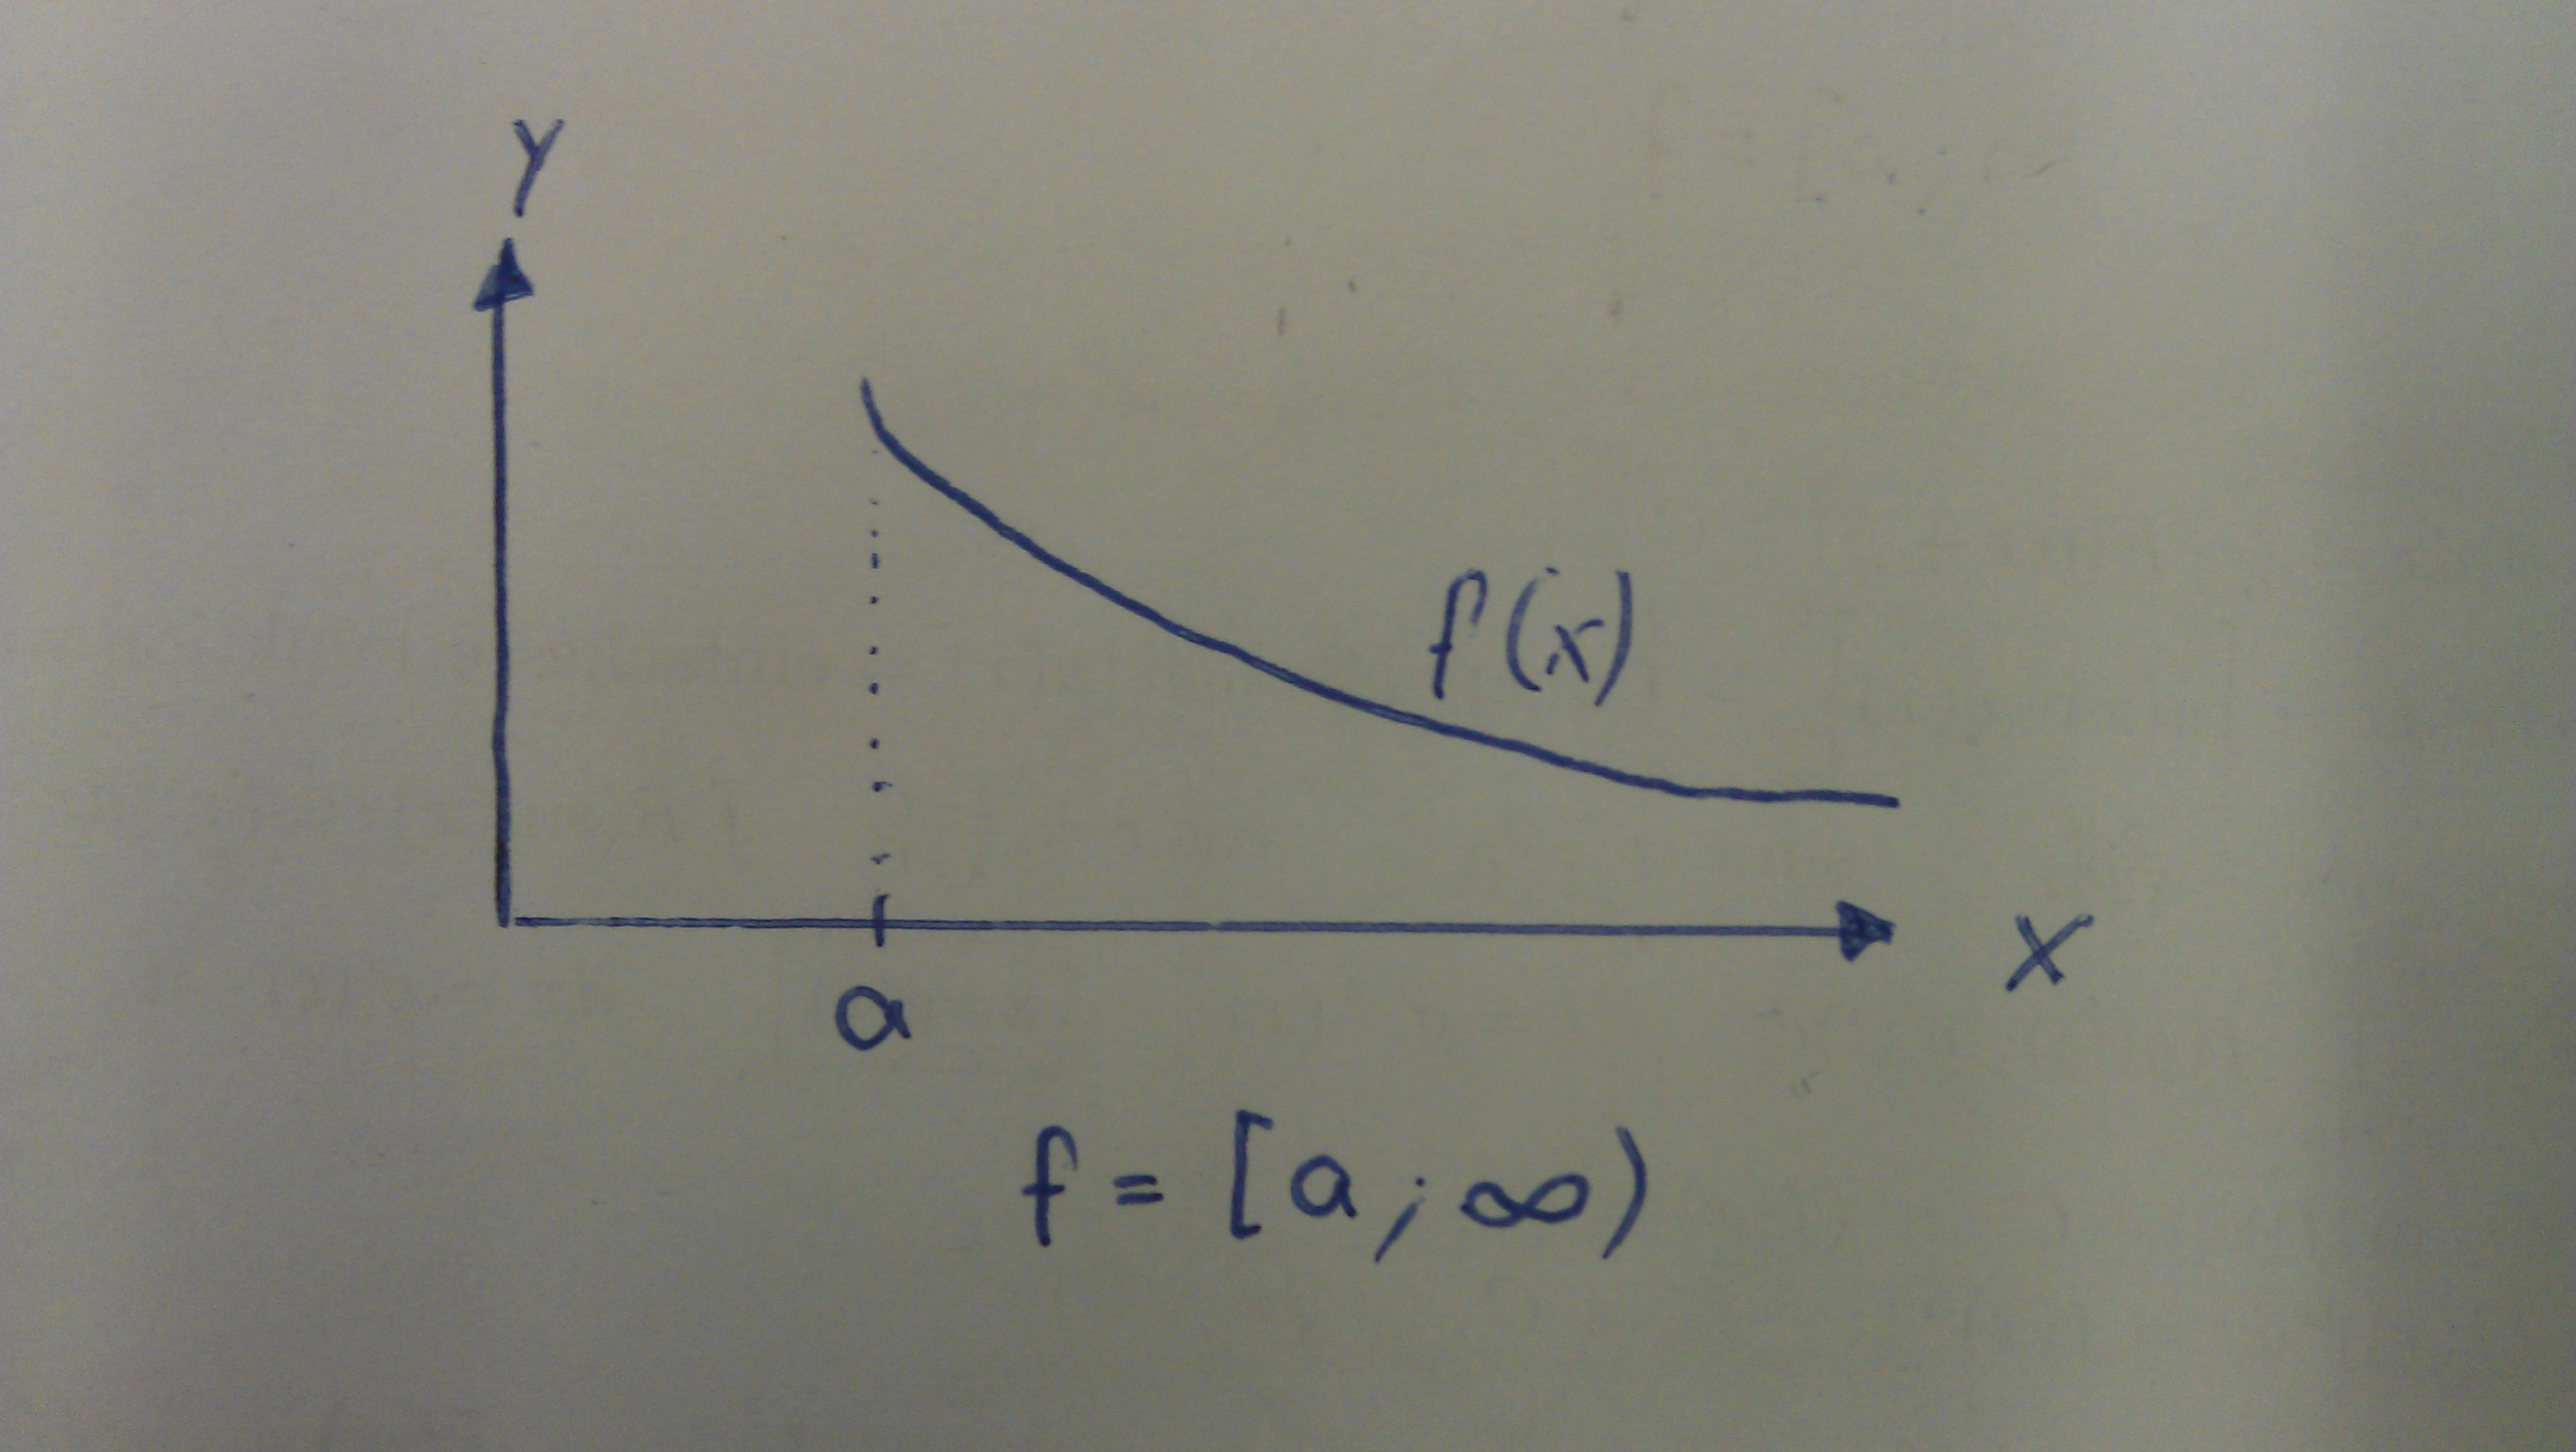
\includegraphics[width = 4cm]{bilder/1_unbeschrint.jpg}}\\
	
	$I =\int\limits _{a}^{c}f(x)dx=	\lim\limits_{t\to b-}\int\limits_{a}^{t}f(x)dx+\lim\limits_{t\to b+}\int\limits_{t}^{c}f(x)dx $& 
	$I =\int\limits _{-\infty} ^{\infty} f(x)dx = \lim \limits_{t_1\to \infty} \lim\limits_{t_2 \to  \infty}\int\limits_{-t_1} ^{a}f(x)dx + \int\limits_{a}^{t_2}f(x)dx $\\

	\hline\hline
	
	Majorantenprinzip (konvergent) & Minorantenprinzip(divergent)\\
	\hline

	Majorante $g(x) \geq f(x) $: Konvergiert $\int\limits_a^{\infty} g(x) dx$, \newline dann konvergiert auch $\int\limits_a^{\infty} f(x) dx$. ($x \in [a, \infty)$)  &
	
	Minorante $g(x) \leq f(x) $: Divergiert $\int\limits_a^{\infty} g(x) dx$, \newline dann divergiert auch $\int\limits_a^{\infty} f(x) dx$. ($x \in [a, \infty)$	 \\
	
	\hline\hline
	\multicolumn{2}{|c|}{Cauchy Hauptwert: bei unbeschränkter Funktion, welche Symmetrisch ist. $\Rightarrow$ Nur ein limit}\\
	
	\multicolumn{2}{|c|}{$I=\int\limits_a^b f(x)dx = \lim\limits_{\epsilon \to 0}\left( \int\limits_a^{\xi -\epsilon}f(x)dx + \int\limits_{\xi+\epsilon}^b f(x)dx\right)$}\\
	
	\hline

	\end{tabularx}
	
	\end{center}
	\end{table}
	

